%%%%%%%%%%%%%%%%%%%%%%%%%%%%%% -*- Mode: Latex -*- %%%%%%%%%%%%%%%%%%%%%%%%%%%%
%% uhtest-appendix.tex -- 
%% Author          : Robert Brewer
%% Created On      : Fri Oct  2 16:31:12 1998
%% Last Modified By: Robert Brewer
%% Last Modified On: Mon Oct  5 14:41:05 1998
%% RCS: $Id: uhtest-appendix.tex,v 1.1 1998/10/06 02:07:03 rbrewer Exp $
%%%%%%%%%%%%%%%%%%%%%%%%%%%%%%%%%%%%%%%%%%%%%%%%%%%%%%%%%%%%%%%%%%%%%%%%%%%%%%%
%%   Copyright (C) 1998 Robert Brewer
%%%%%%%%%%%%%%%%%%%%%%%%%%%%%%%%%%%%%%%%%%%%%%%%%%%%%%%%%%%%%%%%%%%%%%%%%%%%%%%
%% 

\chapter{Some Other Results}

\begin{figure}[h]
        \caption{Inversion table depth image from the intel d435 in color at a rotated view to emphasize the 3D capture and how pixels directly behind the line of sight of the sensor to object will show up as invalid dark pixels.}
        \centering
        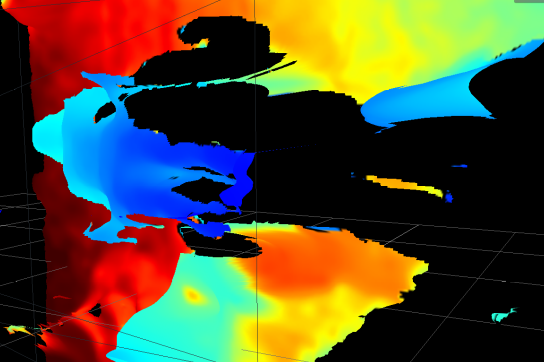
\includegraphics[width=0.5\textwidth]{images/inversion_depth.png}
\end{figure}
 
\begin{figure}[h]
        \caption{Euclidean Error vs. Depth Frame Rate show 30 and 60 frames per second as the best.}
        \centering
        \includegraphics[width=0.7\textwidth]{images/error_depth_frame.png}
\end{figure}
 
\begin{figure}[h]
        \caption{Error vs. Total Color Resolution results show the lowest resolution as the best which hypothetically would be because higher resolution slows down the performance and color is not used for the reconstruction after calibration has been completed.}
        \centering
        \includegraphics[width=0.7\textwidth]{images/error_color.png}
\end{figure}
 

\begin{figure}[h]
        \caption{SPIN 3d reconstruction on single 2d rgb image}
        \centering
        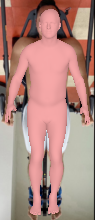
\includegraphics[width=0.2\textwidth]{images/spin.png}
\end{figure}

\begin{figure}[h]
        \caption{SMIL sample output}
        \centering
        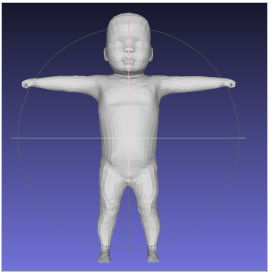
\includegraphics[width=0.4\textwidth]{images/smil.png}
\end{figure}

\begin{figure}[!htb]
        \caption{Missing data in the shape up data}
        \centering
        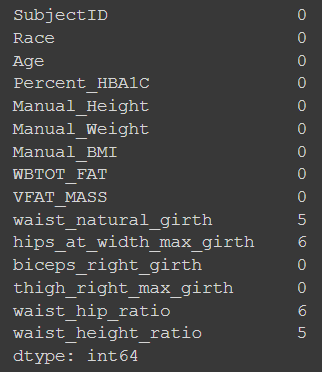
\includegraphics[]{images/missing_data.png}
\end{figure}

\begin{figure}[!htb]
        \caption{HBA1C Distribution in the shape up data}
        \centering
        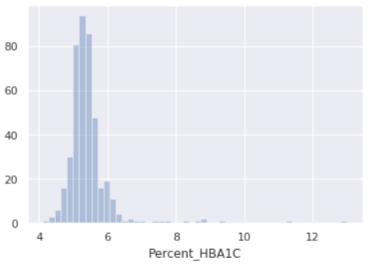
\includegraphics[width=0.5\textwidth]{images/hba1c.png}
\end{figure}

\begin{figure}[!htb]
        \caption{WBTOT FAT Distribution in the shape up data}
        \centering
        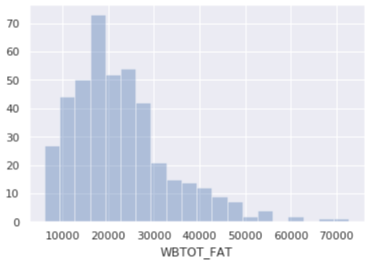
\includegraphics[width=0.5\textwidth]{images/wbtot_fat.png}
\end{figure}


\begin{figure}[!htb]
        \caption{VFAT MASS Distribution in the shapeup data}
        \centering
        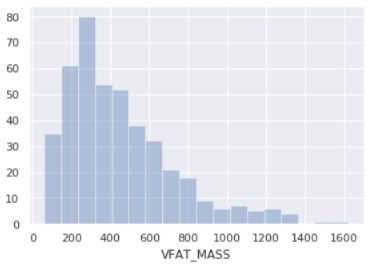
\includegraphics[width=0.5\textwidth]{images/vfat_mass.png}
\end{figure}

\begin{figure}[!htb]
        \caption{Race Ratios Distribution in the shapeup data}
        \centering
        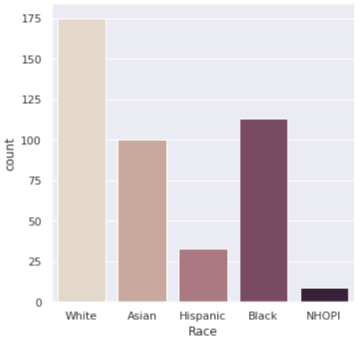
\includegraphics[width=0.5\textwidth]{images/race_ratios.png}
\end{figure}
\begin{figure}[!htb]
        \caption{Fat Mass Training Table using Catboost}
        \centering
        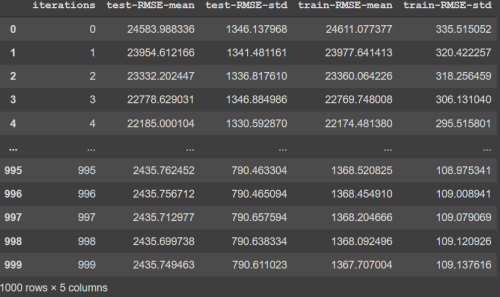
\includegraphics[width=0.7\textwidth]{images/catboost_training.png}
\end{figure}

\begin{table}[!h]
\caption{Mannequin imaging table 1 partial parameters}
\centering
\pgfplotstabletypeset[
    col sep=comma,
    string type,
    columns/.style={column type={|l}},
    columns/.style={column type={|l}},
    columns/.style={column type={|l|}},
    columns/.style={column type={|l}},
    columns/.style={column type={|l}},
    columns/.style={column type={|l}},
    every head row/.style={before row=\hline,after row=\hline},
    every last row/.style={after row=\hline},
    ]{tables/test.csv}
\end{table}


\begin{table}[!h]
\caption{Mannequin imaging table 2 partial parameters}
\centering
\pgfplotstabletypeset[
    col sep=comma,
    string type,
    columns/.style={column type={|l}},
    columns/.style={column type={|l}},
    columns/.style={column type={|l|}},
    columns/.style={column type={|l}},
    every head row/.style={before row=\hline,after row=\hline},
    every last row/.style={after row=\hline},
    ]{tables/test2.csv}
\end{table}

\begin{table}[!h]
\caption{Table of Sensor Accuracy by distance to the sensor (ft)}
\centering
\pgfplotstabletypeset[
    col sep=comma,
    string type,
    columns/.style={column type={|l}},
    columns/.style={column type={|l}},
    columns/.style={column type={|l|}},
    columns/.style={column type={|l}}, 
    columns/.style={column type={|l}},
    columns/.style={column type={|l|}},
    columns/.style={column type={|l}},
    every head row/.style={before row=\hline,after row=\hline},
    every last row/.style={after row=\hline},
    ]{tables/accuracy.csv}
\end{table}
% Setup siunitx:
\sisetup{
  round-mode          = places, % Rounds numbers
  round-precision     = 2, % to 2 places
}
\begin{table}[!h]
\caption{Table of Sensor Temporal Noise by distance to the sensor (ft)}
\centering
\pgfplotstabletypeset[
    col sep=comma,
    string type,
    columns/.style={column type={|l}},
    columns/.style={column type={|l}},
    columns/.style={column type={|l|}},
    columns/.style={column type={|l}}, 
    columns/.style={column type={|l}},
    columns/.style={column type={|l|}},
    columns/.style={column type={|l}},
    every head row/.style={before row=\hline,after row=\hline},
    every last row/.style={after row=\hline},
    ]{tables/temporal-noise.csv}
\end{table}

\begin{table}[!h]
\caption{Table of Fill Rate by distance to the sensor (ft)}
\centering
\pgfplotstabletypeset[
    col sep=comma,
    string type,
    columns/.style={column type={|l}},
    columns/.style={column type={|l}},
    columns/.style={column type={|l|}},
    columns/.style={column type={|l}}, 
    columns/.style={column type={|l}},
    columns/.style={column type={|l|}},
    columns/.style={column type={|l}},
    every head row/.style={before row=\hline,after row=\hline},
    every last row/.style={after row=\hline},
    ]{tables/fill-rate.csv}
\end{table}
\begin{figure}[!htb]
        \caption{Connected Components Best Mesh}
        \centering
        \includegraphics[width=0.2\textwidth]{images/cc_best_mesh_2.png}
\end{figure}
\begin{figure}[!htb]
        \caption{Connected Components Worst  Mesh}
        \centering
        \includegraphics[width=0.2\textwidth]{images/cc_worst_mesh_6.png}
\end{figure}

\begin{figure}[!htb]
        \caption{Best mesh by euclidean distance}
        \centering
        \includegraphics[width=0.2\textwidth]{images/euclidean_ideal.png}
\end{figure}

\begin{figure}[!htb]
        \caption{A fully human labeled mesh, all 300,000 vertices colored by closest caesar landmark}
        \centering
        \includegraphics[width=0.2\textwidth]{images/full_labeled_mesh.png}
\end{figure}

\begin{figure}[!htb]
        \caption{A subsampled human caesar labeled mesh by color}
        \centering
        \includegraphics[width=0.3\textwidth]{images/labeled_mesh.png}
\end{figure}

\begin{figure}[!htb]
        \caption{Ideal mesh reposed through Meshcapade}
        \centering
        \includegraphics[width=0.3\textwidth]{images/reposed_mesh.png}
\end{figure}

\begin{figure}[!htb]
        \caption{Turntable speed non-linear speed}
        \centering
        \includegraphics[width=0.6\textwidth]{images/turntable_time.png}
\end{figure}

\begin{figure}[!htb]
        \caption{Inversion Table Imaging \ang{0}, \ang{30}, \ang{60}, \ang{90} showing visual changes to the body}
        \centering
        \includegraphics[width=0.7\textwidth]{images/en_inversion_di.png}
\end{figure}
\begin{figure}[!htb]
        \caption{Inversion Table Imaging \ang{0}, \ang{30}, \ang{60}, \ang{90} showing visual changes to the body}
        \centering
        \includegraphics[width=0.7\textwidth]{images/mw_inversion_di.png}
\end{figure}
